
\documentclass[]{beamer}
\setbeamertemplate{navigation symbols}{}
%\setbeamertemplate{footline}[title]
\usepackage{beamerthemeshadow}
\usepackage{lastpage}
\usepackage[flushmargin,hang,multiple,ragged]{footmisc}
\usepackage{microtype}
\usepackage{fancyhdr} 


\setbeamertemplate{footline}
{
	\leavevmode%
	\hbox{%
		\begin{beamercolorbox}[wd=.333333\paperwidth,ht=2.25ex,dp=1ex,center]{author in head/foot}%
			\usebeamerfont{author in head/foot}\insertshortauthor
		\end{beamercolorbox}%
		\begin{beamercolorbox}[wd=.333333\paperwidth,ht=2.25ex,dp=1ex,center]{title in head/foot}%
			\usebeamerfont{title in head/foot}\insertshorttitle
		\end{beamercolorbox}%
		\begin{beamercolorbox}[wd=.333333\paperwidth,ht=2.25ex,dp=1ex,right]{date in head/foot}%
			\usebeamerfont{date in head/foot}
		\end{beamercolorbox}}%
	\vskip0pt%
}
%\setbeamertemplate{frametitle}[default][center]
\setbeamercolor{page number in head/foot}{fg=black}
\setbeamerfont{page number in head/foot}{size=\small}
\setbeamertemplate{footline}[page number]
\begin{document}
\title[Meme Emotion Analysis]{\textbf{Memotion Analysis : Automatic processing of Internet Memes} }

\author[SUBALAKSHMI(186001008)]{ \textbf{ Presented By,}\\  SUBALAKSHMI SHANTHOSI S \\(186001008) M.E (CSE) \\~\\  \textbf{Supervised By,} \\ Dr. Aravindan Chandrabose}
%\author{}
\date{\textbf{REVIEW-1 \\ SEPTEMBER 20,2019} }


\begin{frame}
\titlepage
\end{frame}


\begin{frame}\frametitle{Outline}
\begin{itemize}
\item Introduction
\item Motivation
\item Problem statement
\item Literature Survey
\item Existing System
\item Proposed Work
\item Dataset Description
\item References
\end{itemize}
\end{frame}



\begin{frame}\frametitle{Introduction}
\textbf{Memotion Analysis}:\\
\begin{itemize}
\item Automatic processing of internet memes for leveraging meme emotions.\\
Specific intend for detection of offensive memes :To avoid malicious users upload something abusive to torment or disturb people.\\~\\
Need for Meme Emotion Analysis:
\begin{enumerate}
	\item Detection of offensive Meme requires both visual cue and language understanding making them complex to model.\\~\\
	\item No finegrained approach currently existing to distinguish a meme is offensive or humorous.\\~\\
	\item Future exploration on finding differences between Textual and Non-Textual memes on the notion of prominance in sentiment analysis.
\end{enumerate}
 \end{itemize}
\end{frame}
\begin{frame}\frametitle{Introduction(contd...)}
\textbf{Memotion Analysis on Multimodal Social media text}:\\~\\
	 A meme is an idea, behavior, or style that spreads from person to person within a culture—often with the aim of conveying a particular phenomenon, theme, or meaning represented by the meme.\\~\\ Challenges in processing Internet Memes:
\begin{itemize}
	\item A meme is uniquely multimodal because a meme consist of both textual representation and  visual representation. 
	\item Emotion Semantic Image Retrieval(ESIR) with affective gap making the low-level image features extrapolate the high-level semantics.
	\item Replication and mutation of memes.
	\item Challenges on OCR compound as the number of potential fonts,languages,lexicons and other special characters increases. 	
\end{itemize}
\end{frame}



\begin{frame}\frametitle{Motivation}
  Automatic Processing of Internet Memes:
\begin{itemize}
\item  Detection of offensive content on online social media is an ongoing struggle due to voluminous data collected from various sites like Twitter,Facebook,Flickr.
\item  Prevalance of hate speech in social media gives a great societal responsiblity for many social media companies to plan well ahead for mitigation and prevention.
\item Detection of offensive meme is more complex than detecting offensive text as it involves more of language understanding and cognitive psychology.		
\end{itemize}
\end{frame}
\begin{frame}\frametitle{Example Memes}
\begin{center}
	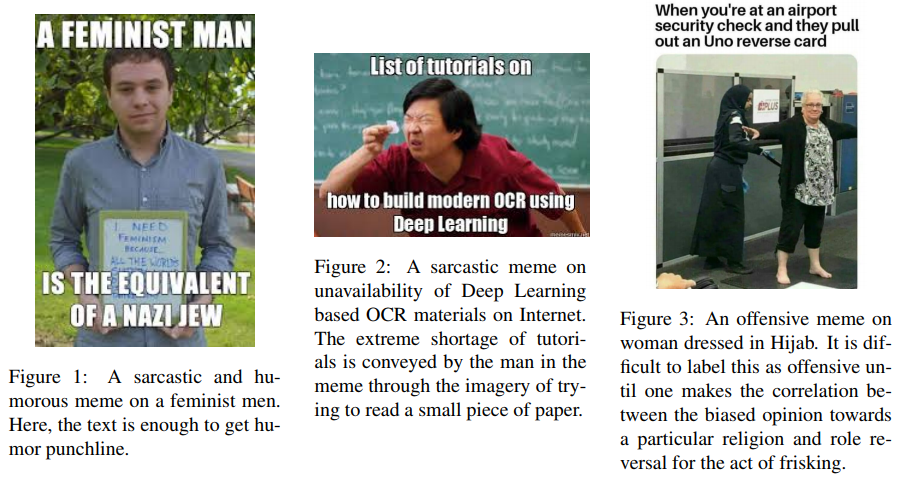
\includegraphics[scale=0.37]{exampleImg/memotion_example.png}
\end{center}
\end{frame}
\begin{frame}\frametitle{Meme Replication and Mutation}
\begin{center}
	
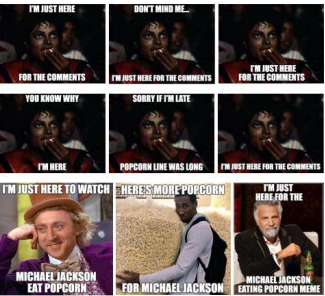
\includegraphics[scale=0.75]{exampleImg/memeRepAndMutation.png}
\end{center}
\end{frame}
\begin{frame}\frametitle{Problem Statement}
  Memes typically induce humor and strive to be relatable. Some memes are directly humorous whereas others go for sarcastic dig at daily life events.Three subtasks varied by the degree of exploration are as follows:
   \begin{enumerate}
	\item  \textbf{Task A - Sentiment Classification}: Given an Internet meme, the first task is to classify it as positive or negative meme. We presume that a meme is not neutral.
	\item \textbf{Task B- Humor Classification}: Given an Internet meme, the system has to identify the type of humor expressed. The categories are sarcastic, humorous, and offensive meme. If a meme does not fall under any of these categories, then it is marked as a other meme. 
	\item \textbf{Task C- Scales of Semantic Classes}: The third task is to quantify the extent to which a particular effect is being expressed(refer Table 1).
\end{enumerate}
\end{frame}
\begin{frame}{Task C - Scales of Semantic Classes}
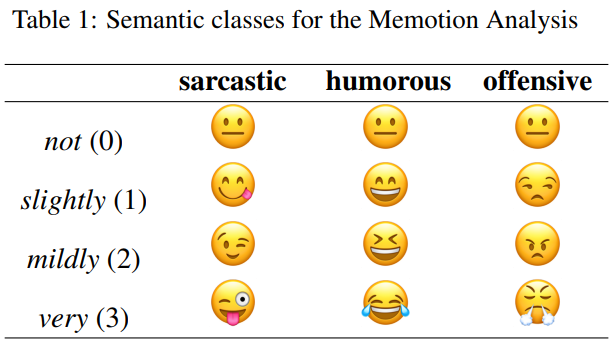
\includegraphics[scale=0.5]{exampleImg/semanticClass.png}
\end{frame}
\begin{frame}\frametitle{Image-based memes as sentiment predictors\cite{imageSentimentPred}}
\begin{columns}
	\begin{column}{0.20\textwidth}
		{\color{blue}{\textbf{Method Used}}}\\
		$\bullet$Finding correlation between Implied semantic meaning and Textual content (discussions).
		$\bullet$Image based descriptor:Visual predictors like colour,depth and shapes.
	\end{column}
	\begin{column}{0.23\textwidth}
		{\color{blue}{\textbf{Results}}}
		\begin{center}$\bullet$Discrepancy in Word level(WL) and phrase level analysis(PL):
		\textbf{Term}:"pixie dust"\\
		\textbf{WL}:"dust"(NEG)\\
		\textbf{PL}:Good luck(Meaning-POS)\\
		$\bullet$ Words with incorrect spelling regarded as NEUTRAL.
	\end{center} 
	\end{column}
\begin{column}{0.20\textwidth}
	{\color{blue}{\textbf{Dataset Used}}}\\
	Facebook:Public posts and discussion\\
	10 discussion forums\\
	997 unique comments
	103 memes
	27,260 words.\\Random discussions pages containing meme
\end{column}
\begin{column}{0.20\textwidth}
	{\color{blue}{\textbf{Advantages}}}\\
	\begin{center}$\bullet$Uncovering challenges like:
	Image at initial conversation shows higher correlation score than text.\\
	$\bullet$More importance to image than text in textual memes.
\end{center}
\end{column}
\begin{column}{0.20\textwidth}
	{\color{blue}{\textbf{Shortcomings and Future Work}}}\\
	\begin{center}
	$\bullet$Misspelled words have NEUTRAL sentiment.\\
	$\bullet$Contradicting word-level and phrase level analysis.
	$\bullet$Sentiment dictionaries required addition of colloquial words.
	\end{center}
\end{column}

\end{columns}
\end{frame}
\begin{frame}\frametitle{ ‘Meme’tic Engineering to Classify Twitter Lingo\cite{memeticEnggTwitter}}
\begin{columns}
	\begin{column}{0.20\textwidth}
		{\color{blue}{\textbf{Method Used}}}
		
		$\bullet$Opinion mining on text meme.\\
		$\bullet$ML Approach: Multinomial Na\"ive Bayes Classifier(MNB) or K-Nearest Neighbours(KNN).\\
		$\bullet$NLP: Text preprocessing using NLTK.
	\end{column}
	\begin{column}{0.23\textwidth}
		{\color{blue}{\textbf{Results}}}
	\textbf{F-Score}
		$\bullet${\color{blue}\textbf{KNN}}:\\
		Positive:70.14\%\\
		Negative:66.32\%\\
		Neutral:66.32\%\\
		$\bullet${\color{blue}\textbf{MNB}}:\\
		Positive:62.29\%\\
		Negative:66.32\%\\
		Neutral:66.32\%\\
		$\bullet$KNN and MNB proves accurate compared to SVM and Logistic Regression.
	\end{column}
	\begin{column}{0.20\textwidth}
		{\color{blue}{\textbf{Datasets}}}\\
		1.Benchmark Dataset:CSV file
		1524 tweets labelled :
		POS(1)\\
		NEG(-1)\\
		NEUTRAL(0)\\
		2.Dynamic Dataset using Twitter API: Tweets gathered for a keyword given by the user.
		\end{column}
	\begin{column}{0.20\textwidth}
		{\color{blue}{\textbf{Advantages}}}
		\begin{center}
		$\bullet$Efficient sentiment evaluator which can be easily integrated to enterprise applications.
		$\bullet$Small scale focused application easier to understand.
		$\bullet$KNN applicable on small dataset.
		\end{center}
	\end{column}
	\begin{column}{0.20\textwidth}
		{\color{blue}{\textbf{Shortcomings and Future Work}}}\\
		\begin{center}
			$\bullet$ Not multilingual compactible.\\
			$\bullet$ OCR Accuracy not taken into account.\\
			$\bullet$ Visual descriptors not given much attention.
		\end{center}
	\end{column}
	
\end{columns}
\end{frame}

\begin{frame}\frametitle{ Meme Opinion Categorization by Using Optical Character Recognition (OCR) and Na\"ive Bayes Algorithm\cite{memeOpinionOCR}}
\begin{columns}
	\begin{column}{0.20\textwidth}
		{\color{blue}{\textbf{Method Used}}}
		
		$\bullet$Opinion Extraction from memes.\\
		$\bullet$Image Processing and NLP methods to classify meme as positive or negative.
		$\bullet$Tesseract OCR is used to extract text from meme.
	\end{column}
	\begin{column}{0.23\textwidth}
		{\color{blue}{\textbf{Results}}}\\~\\
		$\bullet$Accuracy of OCR Tesseract is 75\%.\\
		$\bullet$Na\"ive Bayes algorithm shows fairly good accuracy of 75\%.\\
		$\bullet$Vmap tendency is calculated to find P\textsubscript{max} of all categories of documents tested.
	\end{column}
	\begin{column}{0.20\textwidth}
		{\color{blue}{\textbf{Datasets}}}
		\\$\bullet$ Memes collection: Viral memes towards Indonesian Government.
		$\bullet$ Total number of memes: 100.
		$\bullet$ Train test split: 
		Training Dataset :70 memes.\\
		Test Dataset: 30 memes.
	\end{column}
	\begin{column}{0.20\textwidth}
		{\color{blue}{\textbf{Advantages}}}
		\begin{center}
		$\bullet$ Simple approach\\
		$\bullet$ Vmap to find the P\textsubscript{max} in order to correctly classify testing memes.
		\end{center}
	\end{column}
	\begin{column}{0.20\textwidth}
		{\color{blue}{\textbf{Shortcomings and Future Work}}}
		\begin{center}
			$\bullet$ OCR less accurate: Inability to recognise italics.
			$\bullet$KNN,Neural network can be employed.
			$\bullet$n-gram for enhanced preprocessing.
			
		\end{center}
	\end{column}	
\end{columns}
\end{frame}

\begin{frame}\frametitle{Rosetta: Large Scale System for Text Detection and Recognition in Images\cite{rosettaDataset}}
\begin{columns}
	\begin{column}{0.20\textwidth}
		{\color{blue}{\textbf{Method Used}}}\\
		$\bullet$ Rosetta Facebook's scalable OCR system.
		$\bullet$Two stage process:
		Finding textual region and CNN to recognise text.\\
		$\bullet$ Recognised text stored in TAO for faster search. 
	\end{column}
	\begin{column}{0.23\textwidth}
		{\color{blue}{\textbf{Results}}}\\
		$\bullet$ Error rate of 37\% still recoverable by changing single character. \\
		$\bullet$ Finetuning with manually annotated corpus increased accuracy by 48.06\%\\
		$\bullet$ Random jitter introduced for data augmentation.
	\end{column}
	\begin{column}{0.20\textwidth}
		{\color{blue}{\textbf{Datasets}}}\\$\bullet$COCO-Text:
		$\bullet$ 63,000 images.\\
		$\bullet$ 145,000 text instances.\\
		$\bullet$ Train,Test split: 400k images(training)
		and 50k images for testing.\\
		$\bullet$ Human rated dataset is also used.
	\end{column}
	\begin{column}{0.20\textwidth}
		{\color{blue}{\textbf{Advantages}}}
		
			$\bullet$ Robust and accurate OCR capable of processing millions of images per day.\\
			$\bullet$ Faster search from TAO for recognised text.\\
			$\bullet$ Adaptive character based recognition.
	\end{column}
	\begin{column}{0.20\textwidth}
		{\color{blue}{\textbf{Shortcomings and Future Work}}}
		\\	$\bullet$ Resolution of image increases inference time.\\
			$\bullet$ Case sensitive labelling affected performance.\\
	\end{column}	
\end{columns}
\end{frame}

\begin{frame}\frametitle{ An image-text consistency driven multimodal sentiment analysis approach for social media\cite{imageTextConsistency}}
\begin{columns}
	\begin{column}{0.20\textwidth}
		{\color{blue}{\textbf{Method Used}}}\\
		$\bullet$Visual feature detection using Local Binary Pattern.\\
		$\bullet$ Textual Feature extraction: Continuous bag-of-words or skip-gram. 
		$\bullet$ Image-text similarity found.\\
	\end{column}
	\begin{column}{0.23\textwidth}
		{\color{blue}{\textbf{Results}}}\\~\\
		$\bullet$\textbf{F-score}:\\
		$\bullet$ Positive category:0.87\\
		$\bullet$ Negative category:0.89\\
		$\bullet$ Adaptive merging of textual features with State-of-art SentiBank for improved accuracy.
	\end{column}
	\begin{column}{0.20\textwidth}
		{\color{blue}{\textbf{Datasets}}}
		\\$\bullet$ Visual Sentiment Ontology:\\
		$\bullet$ Total number of images: 603.\\
		$\bullet$ Topics:16.
		$\bullet$ Train test split: random shuffling. 
		Training Dataset :400 images.\\
		Test Dataset: 157 images.
	\end{column}
	\begin{column}{0.20\textwidth}
		{\color{blue}{\textbf{Advantages}}}
		\begin{center}
			$\bullet$ Superior performance in Flickr benchmark dataset.\\
			$\bullet$ Use of Adjective-Noun-Pair(ANP): Converting neutral noun into Strong sentiment word.
		\end{center}
	\end{column}
	\begin{column}{0.20\textwidth}
		{\color{blue}{\textbf{Shortcomings and Future Work}}}
			$\bullet$ SVM modelling unrelated and related data sensitive to outliers.
			$\bullet$ANP difficult due to it's abstract nature and high variability.
	\end{column}	
\end{columns}
\end{frame}

\begin{frame}\frametitle{Existing System}
 \begin{itemize}
 	\item The existing approaches have used meme discussion text correlation and 5-pre trained CNN model for extracting top 10 tags from image individually. \cite{imageSentimentPred}\cite{imageTextConsistency}.
 	\item Rosetta method of Extraction and pre-processing for additional data set creation can be done for multilingual memotion analysis\cite{rosettaDataset}
 	\item KNN or Na\"ive Bayes classifier can be used for maximising F-score.\cite{memeOpinionOCR}\cite{memeticEnggTwitter}. 	
\end{itemize}
\end{frame}

\begin{frame}\frametitle{Proposed Work}
  
\begin{itemize}
\item Pre-trained CNN to work on either image or OCR extracted text based on the image-text correlation.
\item Increasing working dataset size by using Rosetta Facebook's OCR system to make the system more generic by handling multiple languages.
\item KNN approach or Na\"ive Bayes classifier for opinion extraction to categorise as positive or negative.
\item Using ResNet for faster computation.
\end{itemize}
\end{frame}

\begin{frame}\frametitle{Dataset Description}
 \begin{itemize}
 \item 8000 Human Annotated Internet Memes.\\~\\
	
	Input File: \textbf{data.csv} consists of entries: 
	\begin{itemize}
\item Image\_name
\item Image\_URL
\item OCR\_extracted\_text
\item Corrected\_text
\item Humour
\item Sarcasm
\item Offense
\item Motivation
\item Overall\_sentiment
\item Basis\_of\_classification(text or image)   
	\end{itemize}
\end{itemize}
\end{frame}

\begin{frame}\frametitle{References}
\begin{thebibliography}{99}
    \bibliographystyle{plain}
	\bibitem[1]{imageSentimentPred}Jean H. French,{\em Image-based memes as sentiment predictors.}International Conference on Information Society (i-Society), 2017.
	
	\bibitem[2]{memeticEnggTwitter}S. Priyashree, N. Shivani, D. K. Vigneshwar,S. Karthika, {\em International Conference on Computational Intelligence in Data Science(ICCIDS)}, 2017.
	
	\bibitem[3]{memeOpinionOCR}Amalia Amalia , Arner Sharif , Fikri Haisar , Dani Gunawan , Benny B Nasution ,{\em Meme Opinion Categorization by Using Optical Character Recognition (OCR) and Na\"ive Bayes Algorithm.} Third International Conference on Informatics and Computing (ICIC), 2018.
\end{thebibliography}
\end{frame}
	
\begin{frame}\frametitle{References}
	\begin{thebibliography}{99}	
	\bibitem[4]{rosettaDataset} Bogdan Lazarescu, Christo Lolov , Silvia Sapora, {\em Rosetta: Large scale system for text detection and recognition in images.}, 
	KDD'18 Proceedings of the 24th ACM SIGKDD International Conference on Knowledge Discovery and Data Mining,Pages 71-79,2018.
	\bibitem[5]{imageTextConsistency}Ziyuan Zhao , Huiying Zhu , Zehao Xue and Zhao Liu  et al.,{\em An image-text consistency driven multimodal sentiment analysis approach for social media} , Information Processing and Management Vol 56-Issue 6,2019.
\end{thebibliography}
\end{frame}

\begin{frame}
    \begin{LARGE}
    \begin{Huge}
    \begin{center}
        \textbf{THANK YOU}
    \end{center}  
    \end{Huge}  
    \end{LARGE}
  
  
\end{frame}

\end{document}